\chapter{Introduction to Stream and Block Ciphers}

\section{The problem with Vernam cipher}

There are few issues: generating a truly random key as long as the message, find a secure channel for transportation of the key to the message recipient and do this for every single message to be exchanged. In summary, the problem becomes to securely transfer large quantities of secure keys. There are two approaches that are seen as an improvement to Vernam cipher: stream ciphers and block ciphers.


\section{Symmetric encryption}
In stream ciphers we take a seed (a small vector of a few random bits) that must be kept secret, then build a keystream (a very long sequence of pseudorandom bits), finally xor the keystream with the plaintext bitwise to calculate the ciphertext. The problems are how are we going to generate a perfectly random keys of arbitrary size and how can we replicate the random streams of bytes for decryption.
In block ciphers we use the same key multiple times in a way that does not compromise the cipher. The problems are how can we reuse multiple times the same key without enabling an attacker to perform cipher-text only attacks and how can we avoid attackers to exploit the block structure.

These two ciphers are known as symmetric encryption algorithms, where stream ciphers perform operations in a way such that the plaintext is processed one bit at a time, and the algorithm selects one bit of plaintext, performs a series of operations on it, and then outputs one bit of ciphertext, block ciphers perform operations in a way such that the plaintext is processed in blocks (groups) of bits at a time, and the algorithm selects a block of plaintext bits (typically 64 bits), performs a series of operations on them, and then outputs a block of ciphertext bits.
Notice that a stream cipher can be seen as a block cipher with blocksize set to 1 bit, but there are also stream ciphers that process data in bytes, and hence could be regarded as block ciphers with a block size of 8, as a rule of thumb if the blocksize is less than 64 bits we talk about stream ciphers otherwise we talk about block ciphers.


\subsection{Stream ciphers}
The real work in designing a good stream cipher goes into designing the keystream generator. Keystream generators produce output which appears to be randomly generated, but is actually not randomly generated, these are referred to as pseudorandom generators. In many cases, stream ciphers combine the keystream with the plaintext in more complex ways than a simple bitwise xor operation.

\begin{figure}
	\centering
	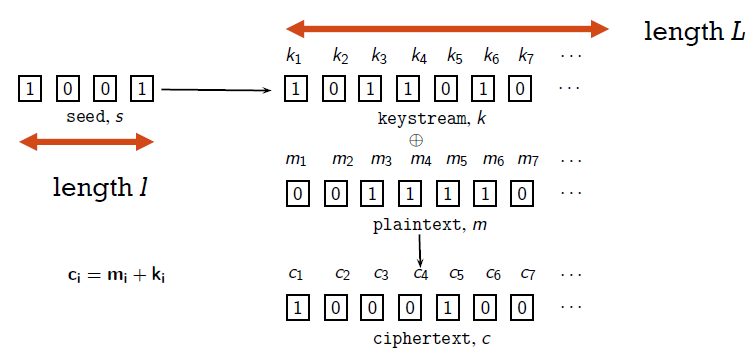
\includegraphics[width=0.7\linewidth]{Images/Chapter2/screenshot000}
	\caption{}
	\label{fig:chapter2_screenshot000}
\end{figure}


For a stream cipher to be good, Eve should not be able to: recover the seed by making the set of possible seeds so large that and exhaustive search is very hard in practice and also predict the rest of the keystream by eliminating any patterns from the keystream.
More precisely: choose a short $l$-bit (much smaller than the lenght L of the plaintext to be encrypted) seed $s$ as the encryption key and stretch the seed into a longer $L$-bit string (the key) that is used  to mask the message and decrypt the ciphertext. The seed $s$ is stretched using some efficient, deterministic algorithm G that maps $l$-bit strings (seeds) to $L$-bit strings(keys). Formally:
\begin{itemize}
	\item Encryption: $G(s)+m$ for any seed s (of size l) and plaintext m (of size L)
	\item Encryption: $G(s) + c$ for any seed s (of size l) and ciphertext c (of size L) where $G$ is called a pseudo-random generator
\end{itemize}

Notice that if $l<L$, then by Shannon’s Theorem, stream ciphers cannot be perfect, however, if G has certain properties, then stream ciphers are secure in practice. Suppose $s$ is a random $l$-bit string and $r$ is a random $L$-bit string, if Eve cannot effectively tell the difference between $G(s)$ and $r$, then it should not be able to tell the difference between stream ciphers and one-time pad. Since the one-time pad latter cipher is secure, so should be the stream cipher.

A stream-cipher is well equipped to encrypt a single message from Alice to Bob. If two messages are encrypted with the same key there may be problems. As an example consider the case in which Alice and Bob want to exchange messages $m_1$ and $m_2$, let $c_1 = m_1 + G(s)$ and $c_2 = m_2 + G(s)$. If Eve is able to intercept both ciphertexts, then it is able to calculate $c_1 + c_2 = ( m_1 + G(s)) + (m_2 + G(s)) = (m_1 + m_2) + (G(s) + G(s)) = m_1 + m_2$, and as english text contains enough redundancy that given $m_1 + m_2$, Eve can recover both m1 and m2 in the clear by using frequency analysis.

Stream-ciphers are said to be malleable since an attacker can cause predictable changes to the plaintext, this is because and attacker can intercept ciphertext $c$ and forwarding $c^'=c+d$, effectively the receiver will get $m' = c' + G(s)= (c+d) + G(s) = (c+G(s)) + d = m + d$. In other words knowing neither $m$ nor $s$, Eve was able to cause the decrypted message to become $m + d $ for $d$ of its choice.

In summary stream-ciphers do not give rise to error propagation as each bit in the ciphertext depends on just one bit in the plaintext and 1 bit transmission errors will result in 1 bit error in the plaintext, also they are very fast making them ideal for real time applications (e.g., mobile communication services) and easy to implement in hardware and don't require large memory capabilities. Since stream ciphers process data bitwise, it is crucial that sender and receiver keep their keystreams in perfect synchronization and 1 bit data loss may have catastrophic consequences as decryptions are performed on the wrong bits after the receiver is out of sync of the sender and re-synchronization mechanisms must be put in place to avoid these problems.


\subsection{Vigenère cipher}

It can be seen as a variant of Vernam cipher whereby the key is a sequence of bits of fixed length. The key, and plaintext are a string of bytes, to encrypt: XOR each character in the plaintext with the next character of the key and wrap around in the key as needed.

Vigenere cipher can be attacked by first determining the key length and determining each byte of the key by using frequency analysis.

\subsection{Block ciphers}

Replace a block of N bits from the plaintext with a block of N bits from the ciphertext. 
\begin{figure}
	\centering
	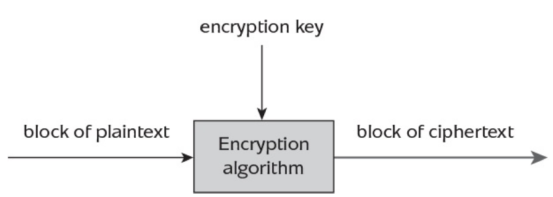
\includegraphics[width=0.7\linewidth]{Images/Chapter2/screenshot001}
	\caption{}
	\label{fig:chapter2_screenshot001}
\end{figure}

\begin{figure}
	\centering
	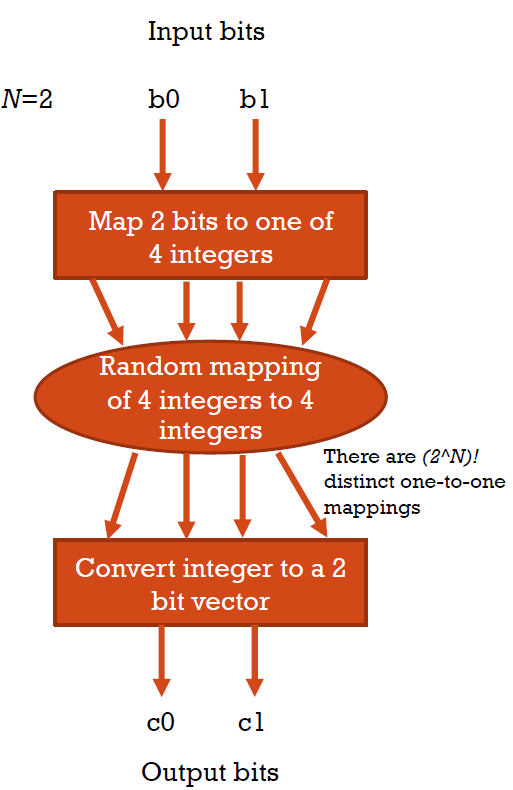
\includegraphics[width=0.4\linewidth]{Images/Chapter2/screenshot002}
	\caption{}
	\label{fig:chapter2_screenshot002}
\end{figure}

The relationship between the input blocks and the output block is completely random. It must be invertible for decryption to work. Thus, it has to be one-to-one, i.e. each input block is mapped to a unique output block. Usually, N=64, 128, 256. If the block size is too small, then the number of different plaintext blocks that can ever be encrypted may be too small for an attacker to launch a type of dictionary attack by building up a dictionary of plaintext/ciphertext pairs, if the block size is too large, then the block cipher becomes inefficient to operate, particularly for plaintexts smaller than the block size as they need padding. The encryption key for the ideal block cipher is the table (also called the codebook) that shows the relationship between the input and the output blocks. Think of each possible input block as one of $2^N$ integers and for each such integer we can specify an output $N$-bit block. If $N$ is 64 then the codebook will be of size $N*(2^N)$ which is around $10^(21)$, but this is not practical since we can can not share such keys.

To make this practical a block cipher is a keyed family of pseudorandom permutations For each key, we have a single permutation that is independent of all the others. Think of each key as corresponding to a different codebook and our strategy is to choose $2^K$ permutations uniformly at random from the set of all $(2^N)!$ permutations

Block ciphers are slower than stream ciphers but are generally considered more secure than the latter.
Block ciphers have a property called diffusion: 2 blocks differing in a single bit shall generate 2 very different ciphertexts. So even a small transmission error will give rise to errors in around half of the bits in the plaintext.


\section{Examples of symmetric ciphers}

\begin{figure}
	\centering
	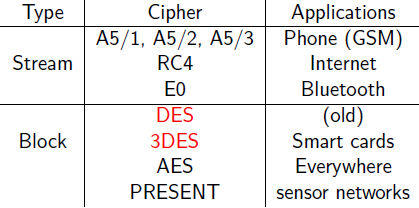
\includegraphics[width=0.7\linewidth]{Images/Chapter2/screenshot003}
	\caption{}
	\label{fig:chapter2_screenshot003}
\end{figure}

\subsection{Examples of stream ciphers}
\begin{itemize}
	\item RC4: Simple and fast stream cipher with a relatively low level of security, probably the most widely implemented stream cipher in software and widely used in SSL/TLS, WEP, and Microsoft Office
	\item A5/1: One of the stream cipher algorithms used in GSM to secure the communication channel over the air from a mobile phone to the nearest base station
	\item E0: The stream cipher algorithm used to encrypt Bluetooth communications
\end{itemize}

\subsection{Examples of block ciphers}

\begin{itemize}
	\item DES: The default block cipher of the 1980s and 1990s, but now considered broken due primarily to its small key size. The two variants based on repeated DES applications commonly known as 3DES are still respected block ciphers, although there are now faster block ciphers available.
	\item AES: A default block cipher based on the encryption algorithm Rijndael which won the AES design competition by NIST to identity the successor of DES
	\item Serpent: A respected block cipher with a block size of 128 bits and key lengths of 128, 192, or 256, which was a finalist with AES in the NIST competition. Considered slower but somehow more secure than AES but not as widely adopted
\end{itemize}

\section{Implementation of stream ciphers}

First we want to tackle the problem of generating a randomly a key (known as keystream )that is as long as possible. Keystream generators should be fast (as in computable in polynomial time as function of number $l$ of bits in the seed) and be secure, so intuitively, a string of L bits produced by a keystream generator should look random. I.e. it should be impossible in a polynomial amount of time in l to distinguish between a truly random bit string of length L and a string of the same length returned by the keystream generator. The main components are:
\begin{itemize}
	\item States: vector of bits organized in registers
	\item Update function: function mapping a state to the next state (clock function)
	\item Output function: function extracting a bit from a state. Concatenating all bits returned by this function, it is possible to obtain the keystream
	\item Key loading: function that takes the seed (secret) and a (public) Initialization Vector (IV) to compute the initial state for the update function. Each IV should be used only once.
\end{itemize}

\begin{figure}
	\centering
	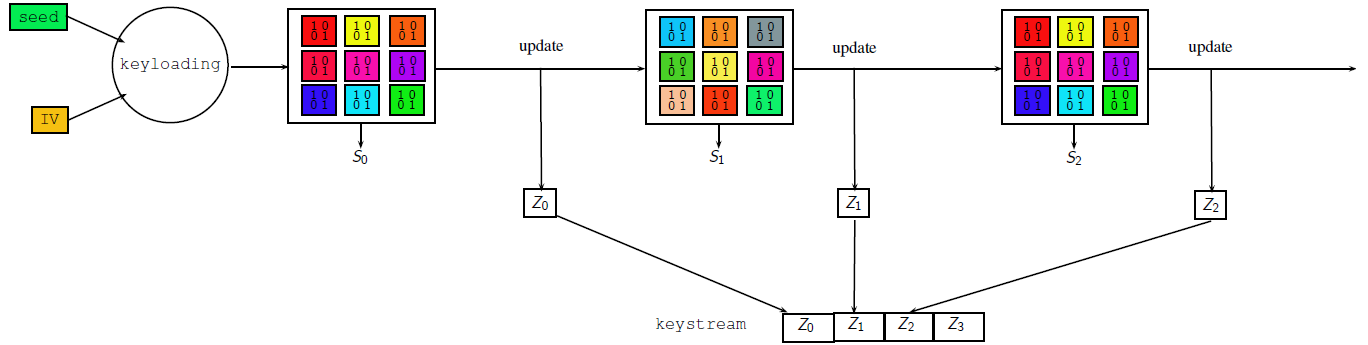
\includegraphics[width=0.9\linewidth]{Images/Chapter2/screenshot004}
	\caption{}
	\label{fig:chapter2_screenshot004}
\end{figure}

\section{Warm Up}

The first output bits strongly depend on the initial state. To avoid potential problems, it is customary to run a warm-up phase before starting encryption. This preliminary phase consists in applying the update function several times without outputting any bits of keystream and it is a highly recommended security best practice.
Given any initial state, the states are periodic, since they are in a finite number and at some point we will obtain again one of the previous states. The keystream is also periodic... this is impossible to avoid. The smallest number $i$ such that $update(...(update(S)))=S$ is called the period of the keystream (it depends on the initial state), and as a requirement is that the period of the keystream shall be quite large, regardless of the initial state, and can be achieved by a suitable design of the update function.
As an example let's take an un update function as follows $f: (x,y,z) \Rightarrow (y+z,x,y)$. One can see that the repeated application of $f$ to the inital state $(1,0,1)$ will yield $(1,0,1) \Rightarrow (1,1,0) \Rightarrow (1,1,1) \Rightarrow (0,1,1) \Rightarrow (0,0,1) \Rightarrow (1,0,0) \Rightarrow (0,1,0) \Rightarrow (1,0,1)$ with a period of 7.


